\documentclass[11pt,a4paper]{article}
\usepackage[margin=1in]{geometry}
\usepackage[T1]{fontenc}
\usepackage[utf8]{inputenc}
\usepackage{lmodern}
\usepackage{hyperref}
\usepackage{enumitem}
\usepackage{xurl}
\usepackage{tikz}
\usepackage{float}
\usetikzlibrary{arrows.meta, positioning, shapes.geometric}
\hypersetup{colorlinks=true,linkcolor=blue,urlcolor=blue}
\newcommand{\codepath}[1]{\path{#1}}
\tikzset{box/.style={rectangle,draw,rounded corners,align=center,inner sep=3pt,minimum width=36mm},line/.style={-Latex}}

\title{Phase-2 gem5: Deliverable 4 (Golden Micro-kernel Traces)}
\author{Senior Systems Architecture}
\date{\today}

\begin{document}
\maketitle

\section{Technical Description}
Golden micro-kernel traces are deterministic gem5 executions used to anchor correctness trends and replay stability.

\section{Implementation Fulfillment}
Generated using \codepath{Phase-2/riscvbench.py} and platform golden runners (where available):
\begin{itemize}[leftmargin=*]
  \item spike: \codepath{Phase-2/tests/run_spike_golden_pipeline.py}
  \item qemu: \codepath{Phase-2/tests/run_qemu_golden_pipeline.py}
  \item gem5: per-target \codepath{riscvbench.py} + replay suite
\end{itemize}
Status for gem5: Execution and normalization implemented; routine pinned golden publication is still maturing.

\section{Design \& Architecture}
From a systems viewpoint, golden traces are pinned control inputs. They must be versioned and replayable to isolate parser/engine regressions from workload churn.

\subsection*{Function Flowchart}
\begin{figure}[H]
\centering
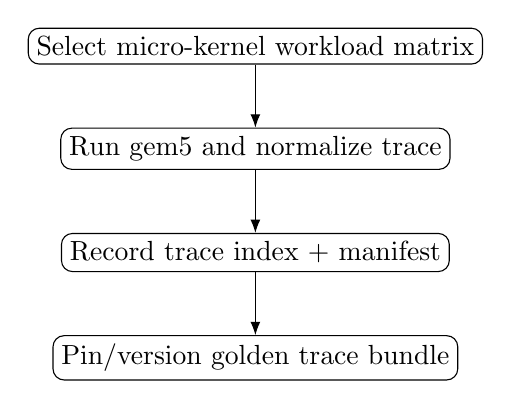
\begin{tikzpicture}[node distance=8mm and 12mm]
\node[box] (a) {Select micro-kernel workload matrix};
\node[box, below=of a] (b) {Run gem5 and normalize trace};
\node[box, below=of b] (c) {Record trace index + manifest};
\node[box, below=of c] (d) {Pin/version golden trace bundle};
\draw[line] (a) -- (b);
\draw[line] (b) -- (c);
\draw[line] (c) -- (d);
\end{tikzpicture}
\caption{gem5 Golden Trace Flow}
\end{figure}

\end{document}
